% Chapter Template

\chapter{Results}
\label{ChapterResults}

This chapter will evaluate how the local search performs compared to the complete algorithm. It will start with a simple iterated local search and show how adding metaheuristics impact the quality of the solution found and the time it takes to return the solution.

\section{Experimental Setup}
All experiments were run on a machine with an Intel Core i7-7700HQ 2.80GHz 64-bit, x64-based processor, 8 GB of DDR4 1200 MHz RAM, and running Windows 10 Home Edition.

\section{Test Data}
The sets of test data are generated using the code described in \cref{random_data_generation}. To test how the algorithms perform as the size of the problem grows, sets of $10, 20, 30, ..., 100$ stories and sprints were generated. Because the data is built randomly, there is the possibility that a data set may be highly constrained or loosely constrained purely by chance. Therefore, 3 different sets of each size are generated and the results are aggregated to control for any variance in the complexity of the data sets.

\Cref{fig:sprints} shows the capacities of the sprints, grouped by how long the road map is (the number of sprints). \Cref{fig:stories} shows how many dependencies the test data sets have, grouped by the size of the product backlog, and \cref{fig:dependencies_stories} shows how complex the backlog is in terms of how many dependencies there are between stories.

\begin{figure}[h!]
    \centering
    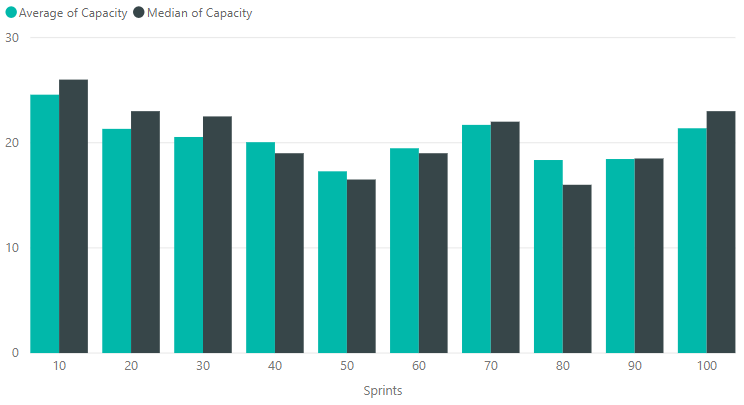
\includegraphics[width=0.8\textwidth]{Figures/TestData/sprints.png}
    \caption{Sprint capacities vs number of sprints}
    \label{fig:sprints}
\end{figure}

\begin{figure}[h!]
    \centering
    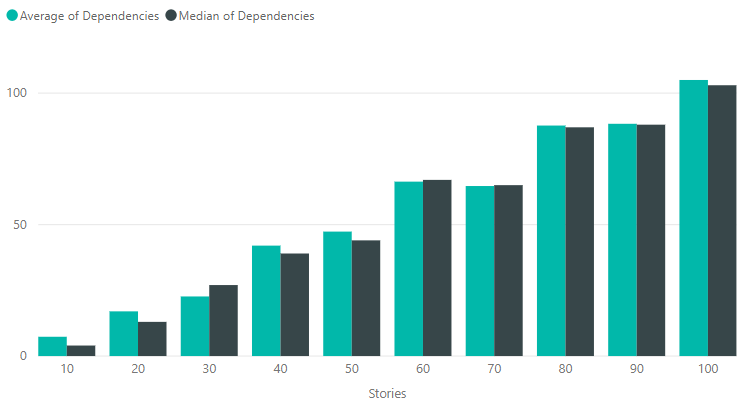
\includegraphics[width=0.8\textwidth]{Figures/TestData/stories.png}
    \caption{Number of dependencies vs number of stories}
    \label{fig:stories}
\end{figure}

\begin{figure}[h!]
    \centering
    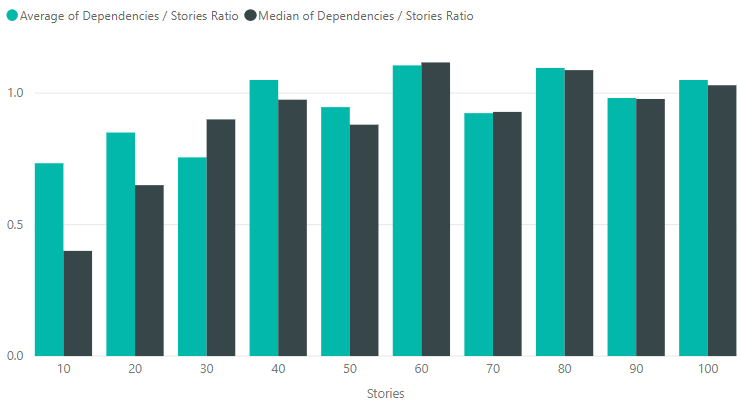
\includegraphics[width=0.8\textwidth]{Figures/TestData/dependencies_stories_ratio.png}
    \caption{Ratio between the number of dependencies and the size of the product backlog}
    \label{fig:dependencies_stories}
\end{figure}

\section{CPLEX Results}

To judge the performance of the local search implementation, the test data was first solved using CPLEX to find the optimal solution to each test problem. The optimal value and the time taken to find it could then be used as a comparison to the local search.

\subsection{Warm vs Cold Starts}

As described in \cref{subsec:warm_start}, CPLEX can use warm starts to improve its performance by giving an initial solution to the Branch and Bound algorithm. This was attempted here and \cref{fig:warm_vs_cold_starts_time} shows that the median time using warm starts was 13\% faster than cold starts. Since this is a very high-level aggregation of the results, it is also interesting to see how warm starts improved the time according to different measures such as the size or difficulty of the problem. \Cref{fig:warm_vs_cold_starts_size} shows that warm starts improved the time across most sizes of problems. \Cref{fig:warm_vs_cold_starts_stories_sprints_ratio} and \cref{fig:warm_vs_cold_starts_dependencies_stories_ratio} similarly show that warm starts matched or improved the time across most difficulties of problems. Therefore in the next section, the metaheuristics results are compared to finding the optimal solution when using warm starts.

\begin{figure}[h!]
    \centering
    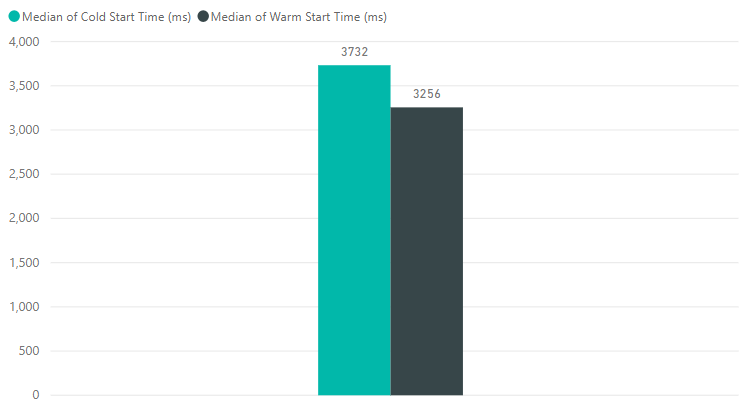
\includegraphics[width=\textwidth]{Figures/WarmVsColdStarts/warm_vs_cold_time.png}
     \caption{Median time using cold starts vs warm starts}
     \label{fig:warm_vs_cold_starts_time}
\end{figure}

\begin{figure}[h!]
    \centering
    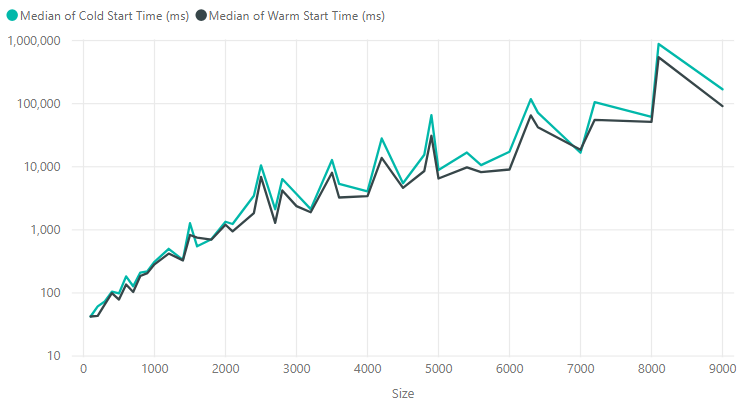
\includegraphics[width=\textwidth]{Figures/WarmVsColdStarts/warm_vs_cold_size.png}
     \caption{Median time of cold starts vs warm starts compared to the size of the problem (shown on a logarithmic scale)}
     \label{fig:warm_vs_cold_starts_size}
\end{figure}

\begin{figure}[h!]
    \centering
    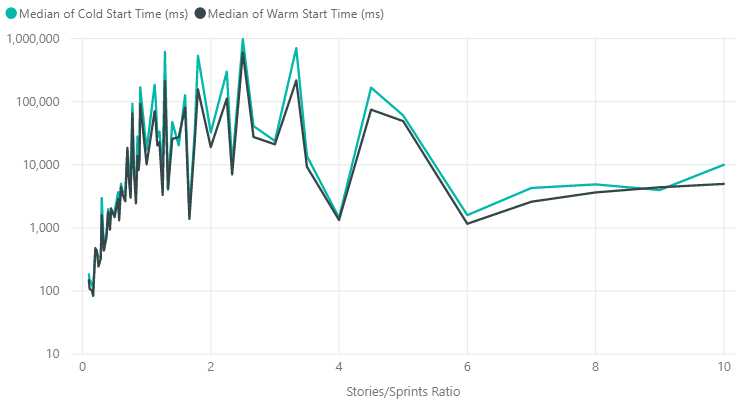
\includegraphics[width=\textwidth]{Figures/WarmVsColdStarts/warm_vs_cold_stories_sprints_ratio.png}
     \caption{Median time of cold starts vs warm starts compared to the ratio of stories to sprints (shown on a logarithmic scale)}
     \label{fig:warm_vs_cold_starts_stories_sprints_ratio}
\end{figure}

\begin{figure}[h!]
    \centering
    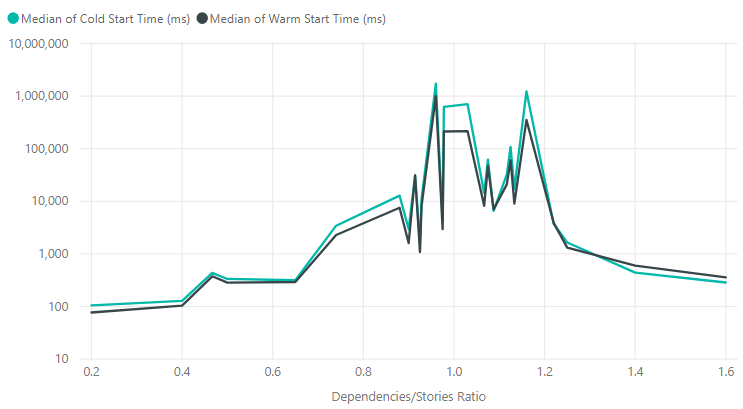
\includegraphics[width=\textwidth]{Figures/WarmVsColdStarts/warm_vs_cold_dependencies_stories_ratio.png}
     \caption{Median time of cold starts vs warm starts compared to the ratio of dependencies to stories (shown on a logarithmic scale)}
     \label{fig:warm_vs_cold_starts_dependencies_stories_ratio}
\end{figure}

\FloatBarrier

\section{Metaheuristic Results}

The metaheuristic algorithm uses randomness at many stages of the search and one execution may produce results that are different to another execution on the same data set. To control for this uncertainty, the metaheuristic algorithm was run 3 times on each test problem and the results are aggregated. To give context to the results, the value gap represents how close the solutions produced by the metaheuristic are, where 0\% means that they are equal (the metaheuristic found the optimal) and 10\% means that the metaheuristic was 10\% below the optimal value. For the time gap, 0\% means that the metaheuristic took exactly the same time as the optimal approach, +10\% means that the metaheuristic was 10\% faster than the optimal approach, and -10\% means that the metaheuristic was 10\% slower than the optimal approach.

Before diving into the comparison of adding each metaheuristic, a summary of the results is given first. The best results were found by using a combination of large neighbourhood search, random restarts and simulated annealing. Adding Tabu search gave slightly worse (but still very good) value solutions in relatively more time than the former combination. When using hill climbing, random restarts and simulated annealing, \cref{fig:value_vs_size} shows that even as the size of the problem grows, the value of solutions found is not significantly impacted and remains close to optimal.

\begin{longtable}[c]{|c|c|}
\caption{Size vs Value gap \% (best and worst highlighted)}
\label{fig:value_vs_size}\\
\hline
\textbf{Size (stories x sprints)} & \textbf{Median Value Gap \%} \\ \hline
\endfirsthead
%
\multicolumn{2}{c}%
{{\bfseries Table \thetable\ continued from previous page}} \\
\hline
\textbf{Size (stories x sprints)} & \textbf{Median Value Gap \%} \\ \hline
\endhead
%
\rowcolor[HTML]{67FD9A} 
100 & 0 \\ \hline
\rowcolor[HTML]{67FD9A} 
200 & 0 \\ \hline
300 & 0.79 \\ \hline
\rowcolor[HTML]{67FD9A} 
400 & 0 \\ \hline
500 & 0.91 \\ \hline
600 & 0.32 \\ \hline
700 & 1.35 \\ \hline
800 & 0.52 \\ \hline
900 & 0.68 \\ \hline
1000 & 1.02 \\ \hline
1200 & 0.41 \\ \hline
1400 & 0.63 \\ \hline
1500 & 0.76 \\ \hline
1600 & 0.49 \\ \hline
1800 & 1.17 \\ \hline
2000 & 0.58 \\ \hline
2100 & 0.78 \\ \hline
2400 & 0.67 \\ \hline
2500 & 0.93 \\ \hline
2700 & 0.9 \\ \hline
2800 & 0.63 \\ \hline
3000 & 1 \\ \hline
3200 & 1.38 \\ \hline
3500 & 0.76 \\ \hline
3600 & 0.91 \\ \hline
4000 & 1.22 \\ \hline
4200 & 0.73 \\ \hline
4500 & 0.63 \\ \hline
\rowcolor[HTML]{FD6864} 
4800 & 1.45 \\ \hline
4900 & 0.53 \\ \hline
5000 & 0.82 \\ \hline
5400 & 0.72 \\ \hline
5600 & 1 \\ \hline
6000 & 0.7 \\ \hline
6300 & 0.59 \\ \hline
6400 & 1.16 \\ \hline
7000 & 0.55 \\ \hline
7200 & 1.13 \\ \hline
8000 & 0.73 \\ \hline
8100 & 1.36 \\ \hline
9000 & 0.79 \\ \hline
10000 & 0.47 \\ \hline
\end{longtable}

Another measure of difficulty is how constrained the problem is. In the ASPP, this can be defined in two ways: the ratio of dependencies to stories, and the ratio of stories to sprints. \Cref{dependencies_stories_ratio_vs_value_gap} shows that the quality of solutions decreases when the ratio of dependencies to stories is close to 1, and \cref{stories_sprints_ratio_vs_value_gap} shows that the solution quality decreases when the ratio of stories to sprints is high. In both cases, this is where the problem is most constrained and the search finds it the most difficult to destroy and repair the candidate solution and may have to traverse through many infeasible solutions before it finds an improving feasible solution.

\begin{table}[h!]
\centering
\begin{tabular}{|c|c|}
\hline
\textbf{Dependencies/Stories Ratio} & \textbf{Median Value Gap \%} \\ \hline
\rowcolor[HTML]{67FD9A} 
0.2 & 0 \\ \hline
\rowcolor[HTML]{67FD9A} 
0.4 & 0 \\ \hline
0.5 & 0.15 \\ \hline
0.7 & 0.2 \\ \hline
0.9 & 0.7 \\ \hline
1 & 1.1 \\ \hline
\rowcolor[HTML]{FD6864} 
1.1 & 2 \\ \hline
1.2 & 1.05 \\ \hline
1.3 & 0.5 \\ \hline
\rowcolor[HTML]{67FD9A} 
1.4 & 0 \\ \hline
\rowcolor[HTML]{67FD9A} 
1.6 & 0 \\ \hline
\end{tabular}
\caption{Dependencies/stories ratio vs value gap \%\\(best and worst highlighted)}
\label{dependencies_stories_ratio_vs_value_gap}
\end{table}

\begin{table}[h!]
\centering
\begin{tabular}{|c|c|}
\hline
\textbf{Stories/Sprints Ratio} & \textbf{Median Value Gap \%} \\ \hline
\rowcolor[HTML]{67FD9A} 
0.1 & 0 \\ \hline
\rowcolor[HTML]{67FD9A} 
0.2 & 0 \\ \hline
\rowcolor[HTML]{67FD9A} 
0.3 & 0 \\ \hline
0.4 & 0.25 \\ \hline
0.5 & 0.1 \\ \hline
0.6 & 0.35 \\ \hline
0.7 & 0.3 \\ \hline
0.8 & 0.55 \\ \hline
0.9 & 0.85 \\ \hline
1 & 0.7 \\ \hline
1.1 & 1 \\ \hline
1.2 & 1.05 \\ \hline
1.3 & 1.5 \\ \hline
1.4 & 1 \\ \hline
1.5 & 1.1 \\ \hline
1.6 & 2.4 \\ \hline
1.7 & 0.9 \\ \hline
1.8 & 1.8 \\ \hline
2 & 2.1 \\ \hline
2.3 & 3.1 \\ \hline
2.5 & 1.9 \\ \hline
2.7 & 4.8 \\ \hline
3 & 3.2 \\ \hline
3.3 & 2.4 \\ \hline
3.5 & 2.6 \\ \hline
4 & 3 \\ \hline
4.5 & 6.2 \\ \hline
5 & 4.6 \\ \hline
6 & 2.4 \\ \hline
7 & 3.6 \\ \hline
8 & 5.2 \\ \hline
\rowcolor[HTML]{FD6864} 
9 & 8 \\ \hline
10 & 3.9 \\ \hline
\end{tabular}
\caption{Stories/sprints ratio vs value gap \%\\(best and worst highlighted)}
\label{stories_sprints_ratio_vs_value_gap}
\end{table}

\FloatBarrier

\Cref{fig:time_vs_size} shows that using the complete method usually terminated faster than the metaheuristic in small problems but the metaheuristic was usually faster in large problems. Similarly, \cref{fig:time_vs_dependencies_stories} and \cref{fig:time_vs_stories_sprints} show that as the complexity of the problems increase, the local search can find close-to-optimal solutions in a similar time in easy problems and much faster in difficult problems.

\begin{figure}[h!]
    \centering
    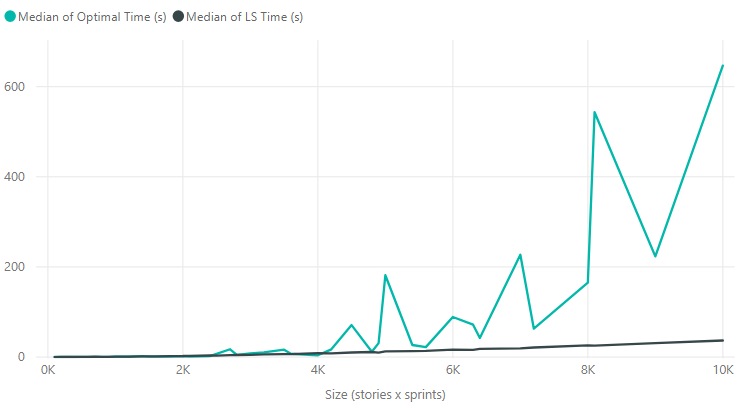
\includegraphics[width=\textwidth]{Figures/FinalResults/annealing_time_size.png}
     \caption{Size vs time - positive gap means the metaheuristic method was faster}
     \label{fig:time_vs_size}
\end{figure}

\begin{figure}[h!]
    \centering
    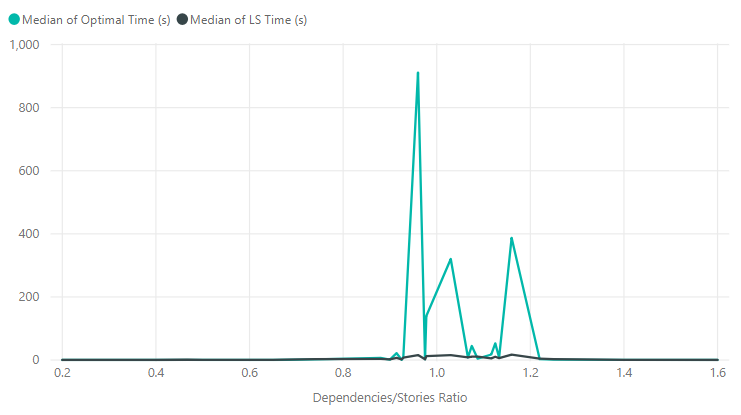
\includegraphics[width=\textwidth]{Figures/FinalResults/annealing_time_dependencies_stories.png}
     \caption{Ratio of dependencies to stories vs time - positive gap means the metaheuristic method was faster}
     \label{fig:time_vs_dependencies_stories}
\end{figure}

\begin{figure}[h!]
    \centering
    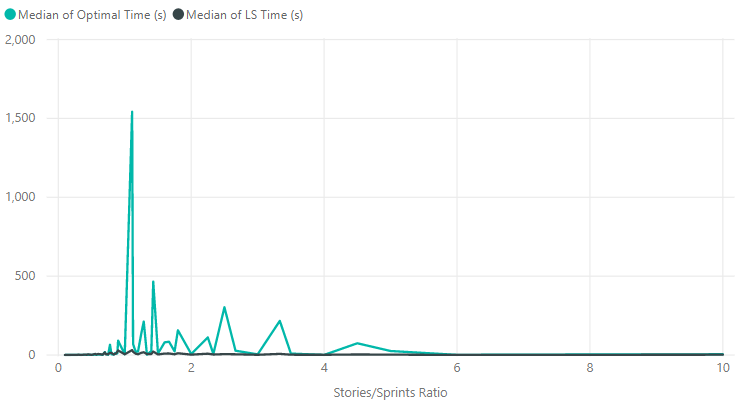
\includegraphics[width=\textwidth]{Figures/FinalResults/annealing_time_stories_sprints.png}
     \caption{Ratio of stories to sprints vs time - positive gap means the metaheuristic method was faster}
     \label{fig:time_vs_stories_sprints}
\end{figure}

\FloatBarrier

\subsection{Comparison of Metaheuristics}

To test how each metaheuristic impacts the value and time of finding approximate solutions, the metaheuristic algorithm was first run using only large neighbourhood search (LNS) where only improving candidate solutions are accepted (also known as hill climbing). Using this is a baseline, other metaheuristic strategies were cumulatively added in the following order: random restarts (restarts), simulated annealing (SA), tabu search (TS). To compare the impact of adding each metaheuristic, \cref{heuristic_gaps} shows the value and time gaps when adding each metaheuristic. It is important to note that these results are aggregated at a high level across problem instances of very different sizes and difficulties and these results are shown only to illustrate the general trend - a more detailed analysis of the results is given in \cref{subsec:result_distributions}. The results shows that even the basic hill climbing can get within 1.65\% (average) / 0.95\% (median) of the optimal value but the standard deviation is relatively high, suggesting that it gives inconsistent results. Adding random restarts closes the value gap to 1.34\% (average) / 0.71\% (median) and takes approximately the same amount of time. This is expected because hill climbing and random restarts were given the same number of iterations, but the latter was allowed to restart up to 10 times within that number of iterations if the search stagnated. Adding simulated annealing slightly improved the value gap but the time gap noticeably worsened. However, the median time gap shows that it still performed 9\% faster than the complete algorithm. Adding tabu search slightly increased the value gap and dramatically increased the time gap.

The small increase in the value gap when using tabu search could be because the search is getting stalled when the tabu list forbids accepting certain moves. Possible reasons for this could be the definition of the move or the length of the tabu tenure. On reflection, a better definition of a move could have been to have the concept of a departure sprint and a destination sprint. The tabu list would then prevent moving a story from its destination sprint back to its departure sprint whereas the definition used in this thesis was only to prevent a story being moved back to its departure sprint (i.e. it could not be moved from \emph{any} sprint back to its departure sprint while it was tabu). It could also be due to the fact that neighbours are generated stochastically and there may be cases where several successive neighbours are generated but all contain the same banned moves. As long as there is the chance that a move that was already recently found to be tabu can appear in successive neighbours (effectively a 'random choice with replacement' approach), the search may stall. On one hand, this is precisely the job of the tabu list so that the search is encouraged to explore new areas, but ultimately, preventing the search from accepting neighbours costs iterations that may have led to higher-value solutions. The worse time gap could simply be due to the additional overhead of creating moves during destruction, checking moves, and generally managing the tabu list. This overheard is low in small problems but since both the size of the tabu list and the tabu tenure are functions of the size of the problem, this overhead grows as the size of the problem grows (although it does only grow linearly). Additionally, \cref{subsec:result_distributions} will show that most 
%%%%%%%%%%%%%%%%%%%%%%%%%%%%%%%%%%%%%%%%%%%%%%%%%%%%%%%%%%%%%%%%%%%%%%%%%%%%%%%%%%%%%%%%%%%%%%%%%%%%%

\begin{table}[h!]
\centering

\begin{tabular}{|l|c|c|c|c|c|c|c|c|}
\hline
 & \multicolumn{4}{c|}{\textbf{Value Gap \%}} & \multicolumn{4}{c|}{\textbf{Time Gap \%}} \\ \hline
\textbf{Heuristics} & \textbf{Min} & \textbf{Avg} & \textbf{Median} & \textbf{Max} & \textbf{Min} & \textbf{Avg} & \textbf{Median} & \textbf{Max} \\ \hline
LNS & 0 & 1.65 & 0.95 & 14.72 & -162.33 & 36.96 & 53.7 & 99.69 \\ \hline
LNS + Restarts & 0 & 1.34 & 0.71 & 9.82 & -161.96 & 37.66 & 53.98 & 99.69 \\ \hline
LNS + Restarts + SA & 0 & 1.34 & 0.69 & 10.88 & -367.49 & -26.04 & 8.51 & 99.43 \\ \hline
LNS + Restarts + SA + TS & 0 & 1.36 & 0.7 & 9.53 & -505.45 & -60.47 & -16.37 & 99.32 \\ \hline
\end{tabular}
\caption{Value and time gaps (positive time gap means the metaheuristic method was faster than the complete method)}
\label{heuristic_gaps}
\end{table}

\subsection{Result Distributions}
\label{subsec:result_distributions}

\Cref{fig:value_gap_perc_hill_climb}, \cref{fig:value_gap_perc_restarts}, \cref{fig:value_gap_perc_annealing} and \cref{fig:value_gap_perc_tabu} show the distribution of the gap between the value and time compared to the complete algorithm when adding each metaheuristic. The interesting result shown by these figures compared to the high-level aggregated results in the previous section is that most solutions were within 1\% in all combinations of metaheuristics. The basic hill climbing was able to find solutions within 0.5\% of the optimal but some were up to 15\% away from the optimal. The key improvement that adding random restarts, simulated annealing and tabu search made is to 'shift' the distribution of the value gaps to the left and the distribution of the time gaps to the right. In other words, while there are still outliers in the value and time gaps, adding the metaheuristics found better solutions in less time in most cases.

\begin{figure}[!htbp]
    \centering
    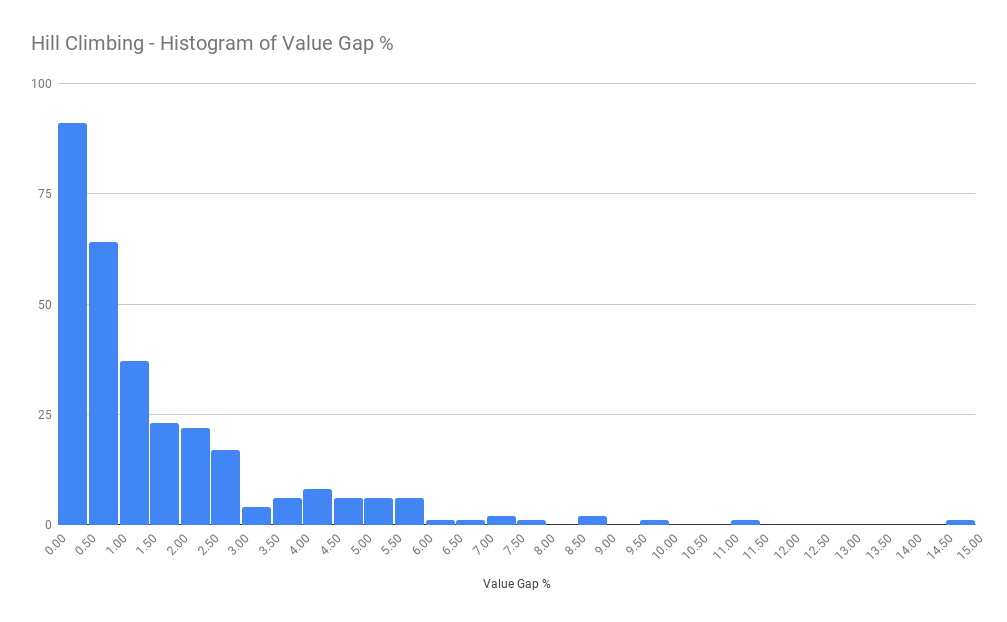
\includegraphics[width=\textwidth]{Figures/Metaheuristics/hill_climb_value_gap.png}
    \caption{LNS (Hill Climbing) Value Gap \%}
    \label{fig:value_gap_perc_hill_climb}
\end{figure}

\begin{figure}[!htbp]
    \centering
    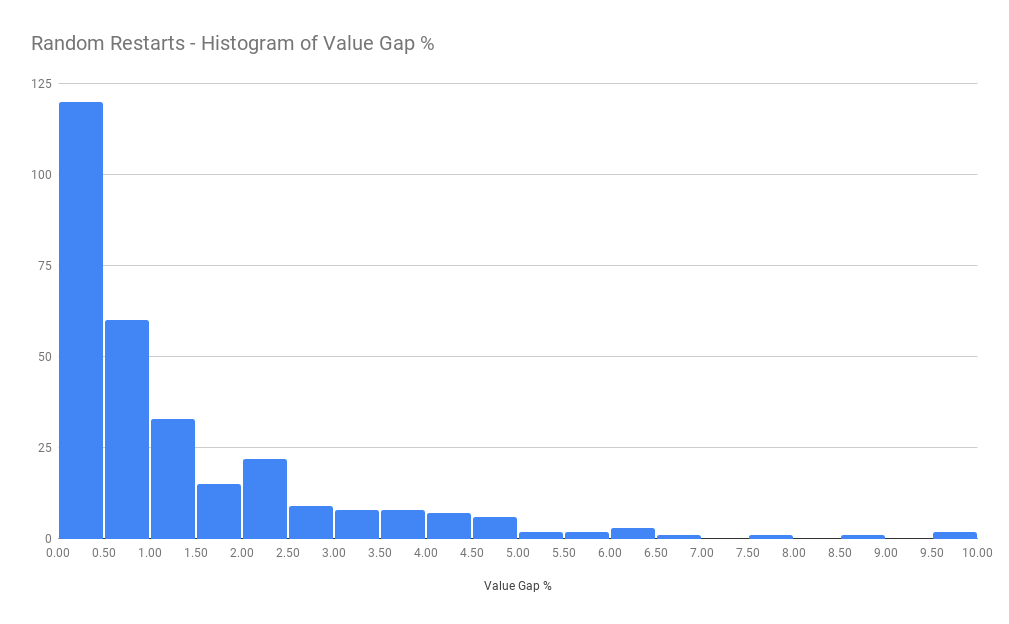
\includegraphics[width=\textwidth]{Figures/Metaheuristics/restarts_value_gap.png}
    \caption{LNS + Random Restarts Value Gap \%}
    \label{fig:value_gap_perc_restarts}
\end{figure}

\begin{figure}[!htbp]
    \centering
    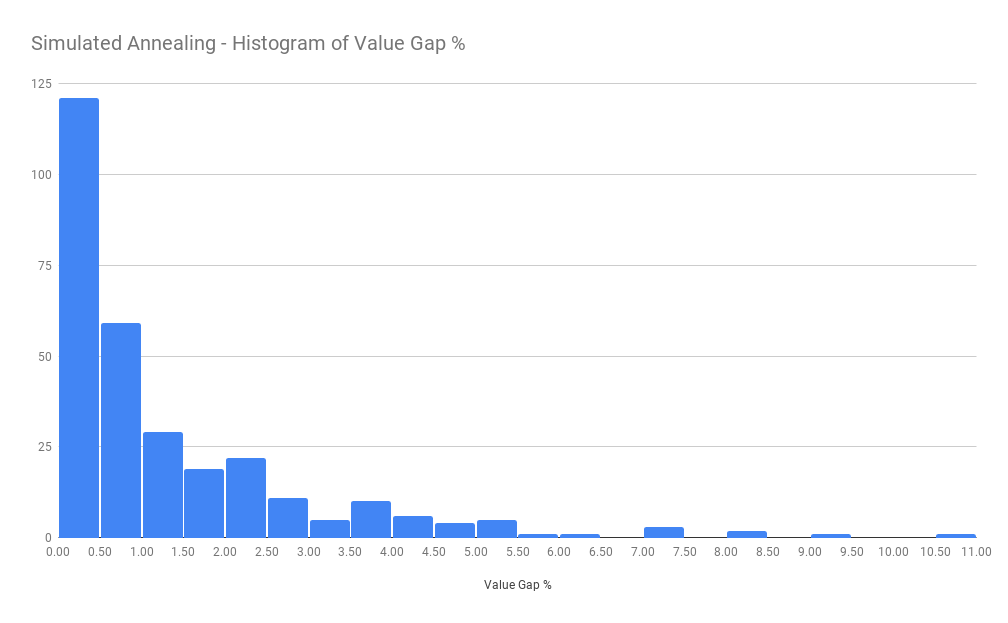
\includegraphics[width=\textwidth]{Figures/Metaheuristics/annealing_value_gap.png}
    \caption{LNS + Random Restarts + SA Value Gap \%}
    \label{fig:value_gap_perc_annealing}
\end{figure}

\begin{figure}[!htbp]
    \centering
    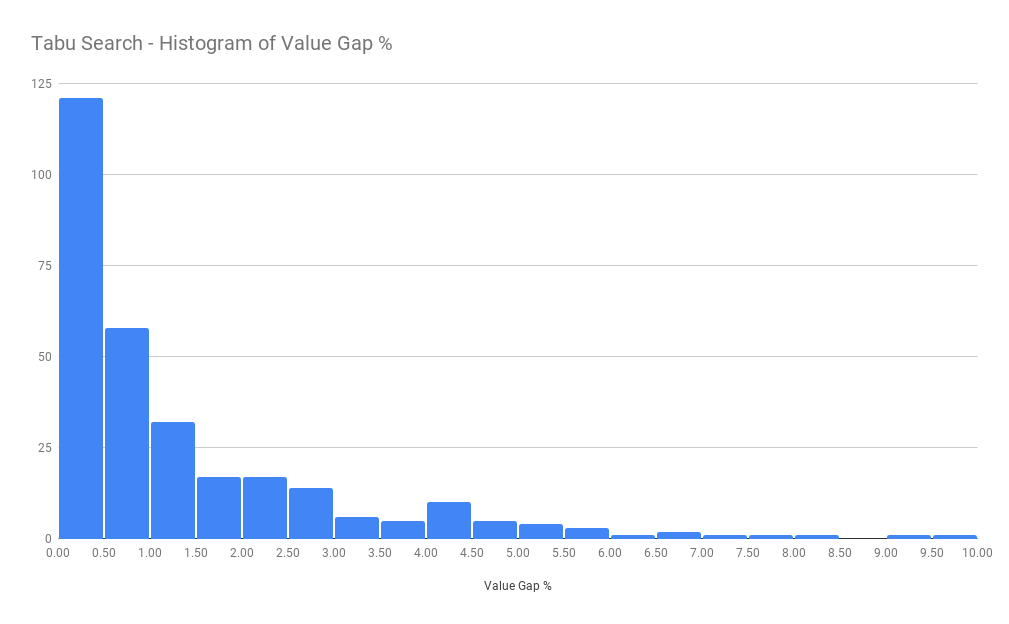
\includegraphics[width=\textwidth]{Figures/Metaheuristics/tabu_value_gap.png}
    \caption{LNS + Random Restarts + SA + TS Value Gap \%}
    \label{fig:value_gap_perc_tabu}
\end{figure}

\begin{figure}[!htbp]
    \centering
    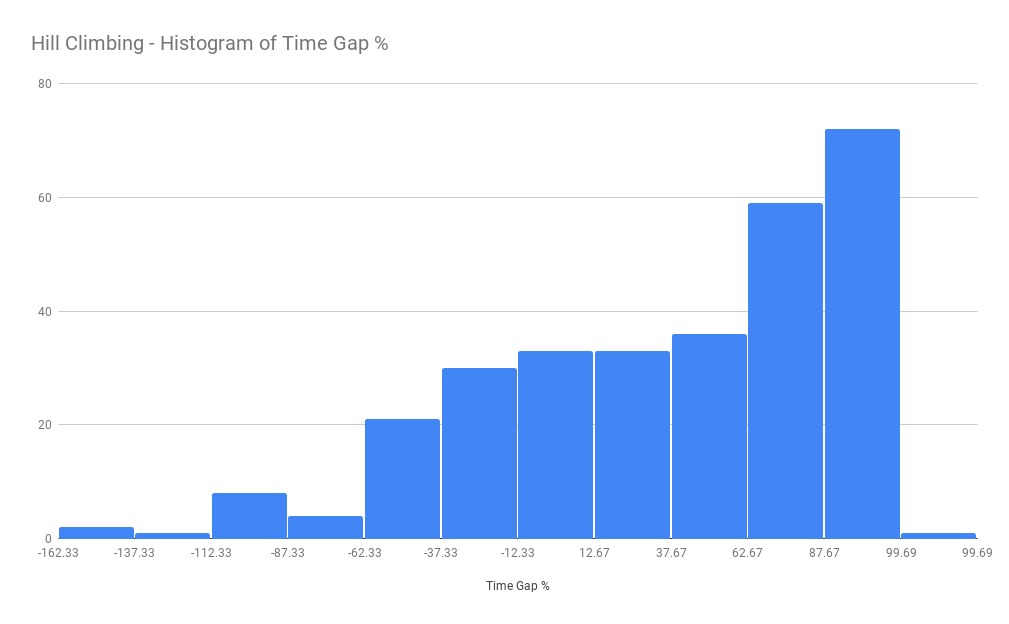
\includegraphics[width=\textwidth]{Figures/Metaheuristics/hill_climb_time_gap.png}
    \caption{LNS (Hill Climbing) Time Gap \% - positive gap means the metaheuristic method was faster}
    \label{fig:time_gap_perc_hill_climb}
\end{figure}

\begin{figure}[!htbp]
    \centering
    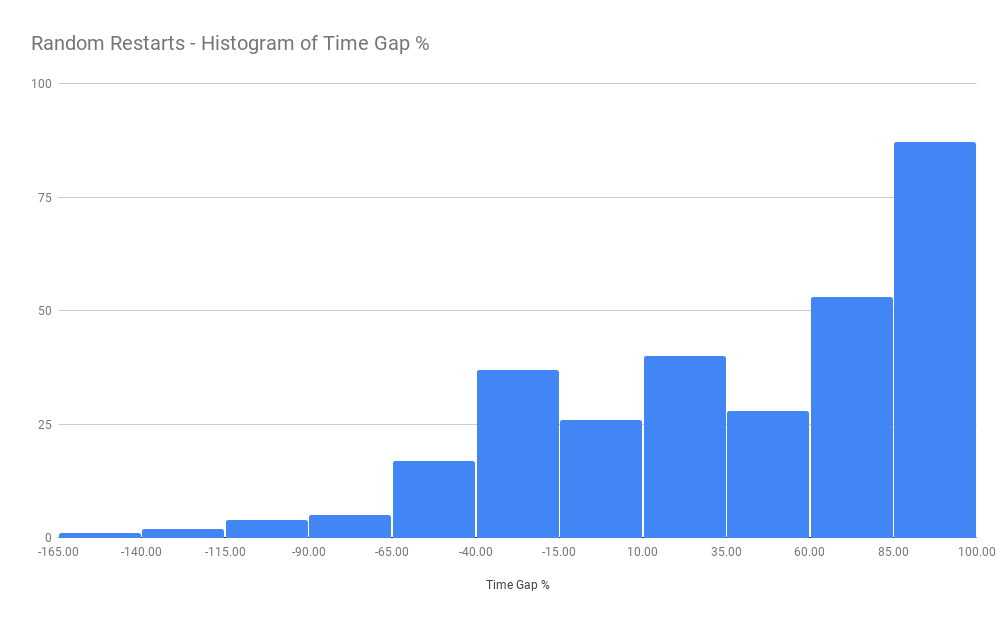
\includegraphics[width=\textwidth]{Figures/Metaheuristics/restarts_time_gap.png}
    \caption{LNS + Random Restarts Time Gap \% - positive gap means the metaheuristic method was faster}
    \label{fig:time_gap_perc_restarts}
\end{figure}

\begin{figure}[!htbp]
    \centering
    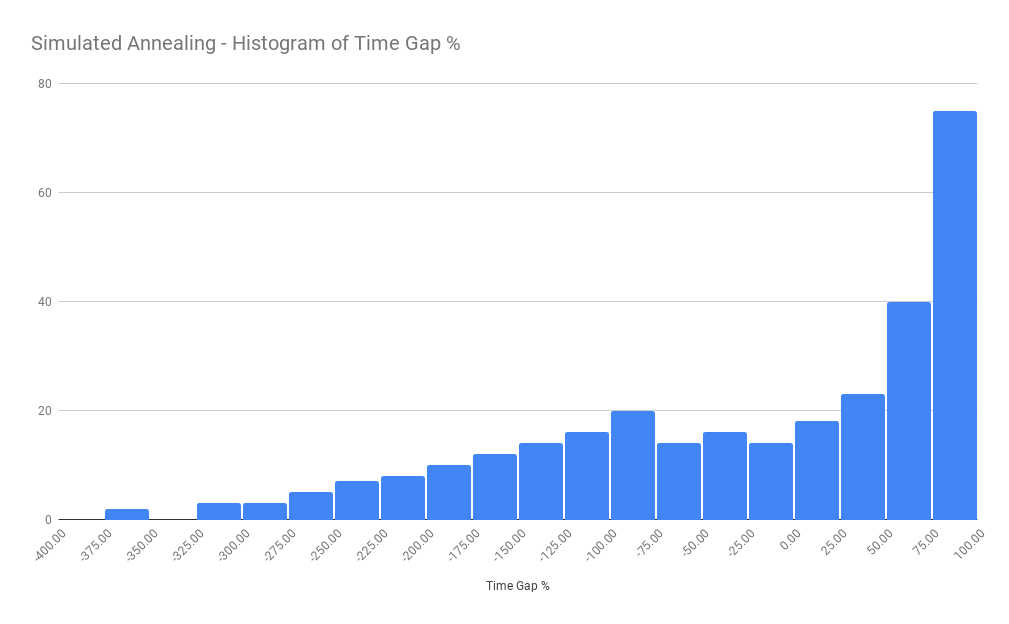
\includegraphics[width=\textwidth]{Figures/Metaheuristics/annealing_time_gap.png}
    \caption{LNS + Random Restarts + SA Time Gap \% - positive gap means the metaheuristic method was faster}
    \label{fig:time_gap_perc_annealing}
\end{figure}

\begin{figure}[!htbp]
    \centering
    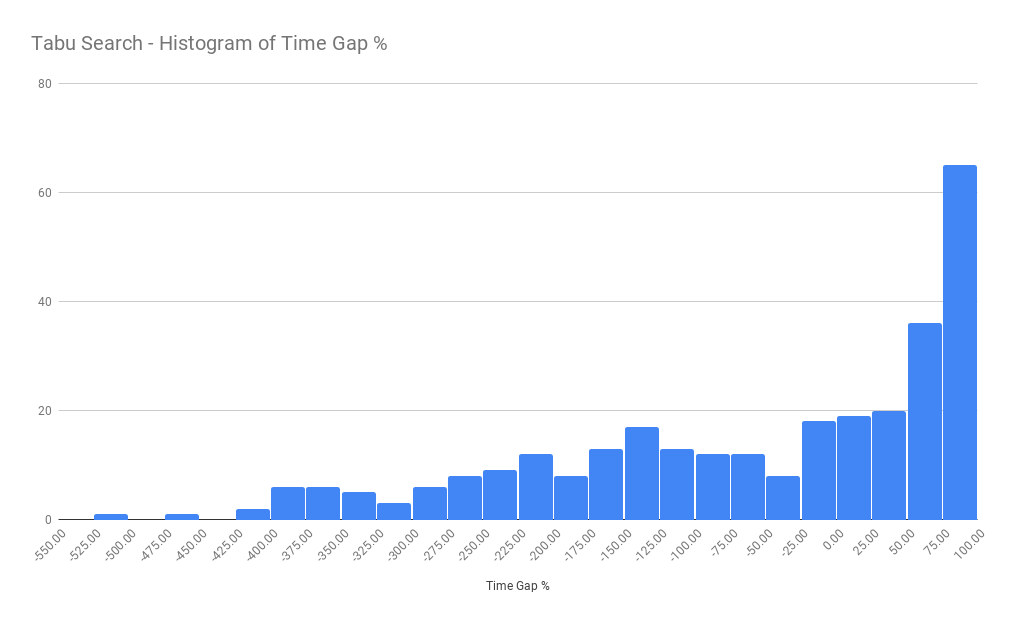
\includegraphics[width=\textwidth]{Figures/Metaheuristics/tabu_time_gap.png}
    \caption{LNS + Random Restarts + SA + TS Time Gap \% - positive gap means the metaheuristic method was faster}
    \label{fig:time_gap_perc_tabu}
\end{figure}

\FloatBarrier

\subsection{Value and Time Gaps}

Even though the search can be seen to perform well overall, it is also important to understand how and why this metaheuristic approach struggles and why the outliers occur. Take note that all figures shown in this subsection are using the combination of LNS (hill climbing), random restarts and simulated annealing since this gave the best results, and they do not include tabu search. As a reminder, the value gap represents how close the solutions produced by the metaheuristic are, where 0\% means that they are equal (the metaheuristic found the optimal) and 10\% means that the metaheuristic was 10\% below the optimal value. For the time gap, 0\% means that the metaheuristic took exactly the same time as the optimal approach, +10\% means that the metaheuristic was 10\% faster than the optimal approach, and -10\% means that the metaheuristic was 10\% slower than the optimal approach.

\Cref{fig:value_gap_vs_size} shows that the value gap is much smaller or finds the optimal solution in small problems and increases in larger problems (fluctuating around 0.74\% in these results). However, it's clear from the time gap in \cref{fig:time_gap_vs_size} that the local search is usually slower than the complete algorithm in small problems but is faster in large problems. Naturally, if the solution space is small, Branch and Bound can traverse most of it in a very short time whereas a local search with a fixed number of iterations may 'waste' some time in these cases.

\begin{figure}[h!]
    \centering
    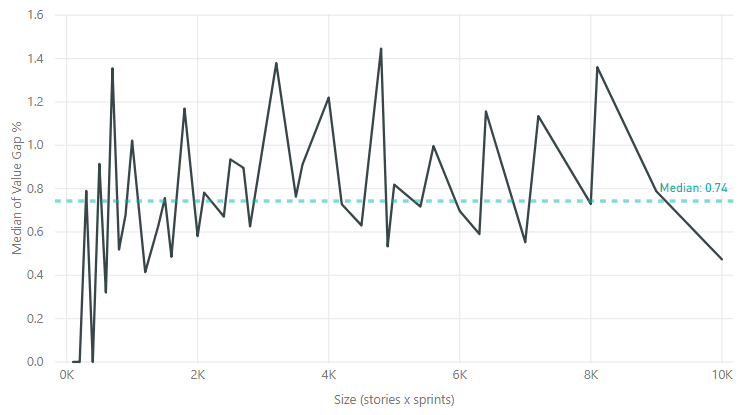
\includegraphics[width=\textwidth]{Figures/Results/annealing_value_gap_size.png}
    \caption{Value Gap \% vs Size}
    \label{fig:value_gap_vs_size}
\end{figure}

\begin{figure}[h!]
    \centering
    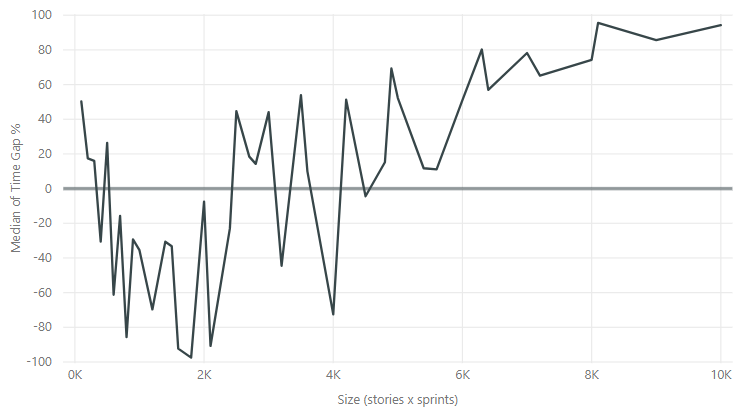
\includegraphics[width=\textwidth]{Figures/Results/annealing_time_gap_size.png}
    \caption{Time Gap \% vs Size}
    \label{fig:time_gap_vs_size}
\end{figure}

For the ratio of dependencies to stories, \cref{fig:value_gap_vs_dependencies_stories} shows that the value gap peaks between 1 and 1.2 where there are roughly the same number of stories and dependencies. This makes sense because problems that have many dependency constraints are difficult to destroy and repair effectively using greedy heuristics as there are fewer feasible ways to insert stories. The time gap in \cref{fig:time_gap_vs_dependencies_stories} shows that the local search is much faster than the optimal search around the 1 to 1.2 range. This could be because the local search is able to find a good, but not necessarily the best, neighbour at each iteration and it is able to continue searching without 'stalling' and can terminate quickly. If the optimal algorithm must find the best set of assignments to make at each iteration, it must spend more time evaluating each step. In other words, when the ratio of dependencies to stories is around 1:1, the local search is able to terminate faster than branch and bound but the value gap increases.

\begin{figure}[h!]
    \centering
    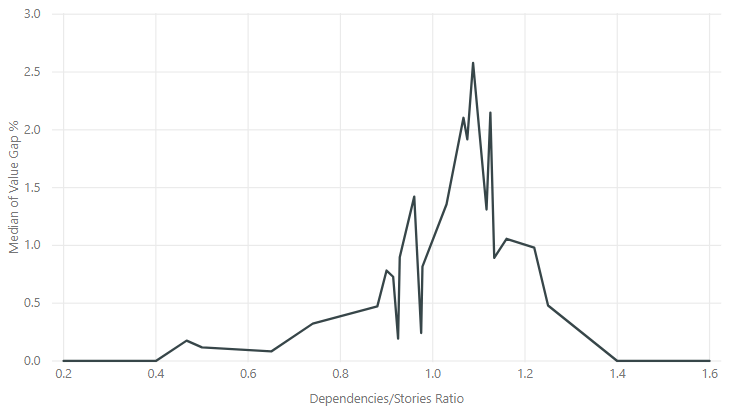
\includegraphics[width=\textwidth]{Figures/Results/annealing_value_gap_dependencies_stories.png}
    \caption{Value Gap \% vs Dependencies/Stories Ratio}
    \label{fig:value_gap_vs_dependencies_stories}
\end{figure}

\begin{figure}[h!]
    \centering
    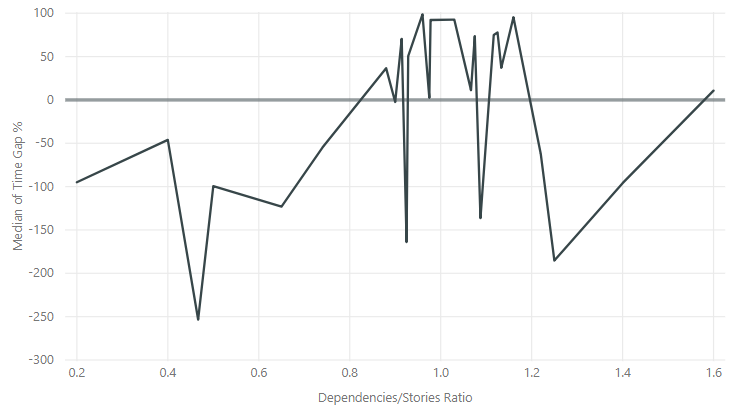
\includegraphics[width=\textwidth]{Figures/Results/annealing_time_gap_dependencies_stories.png}
    \caption{Time Gap \% vs Dependencies/Stories Ratio}
    \label{fig:time_gap_vs_dependencies_stories}
\end{figure}

For the ratio of stories to sprints, \cref{fig:value_gap_vs_stories_sprints} shows that the value gap increases as the ratio increases. This seems to be the largest explanation for the worst solutions found in all of the problems tested in this paper with the median value gap peaking around 8\%. This suggests that this local search is better at solving road maps with a longer time horizon compared to planning many stories into only a few sprints. The time gap shows that the local search generally is slower than the optimal algorithm where the ratio is low and faster it is high. As with the dependencies/stories ratio, this could be because the local search is able to spend less time at each iteration and terminate faster but in the end returns a lower-value solution than in problems where the stories/sprints ratio is low.

\begin{figure}[h!]
    \centering
    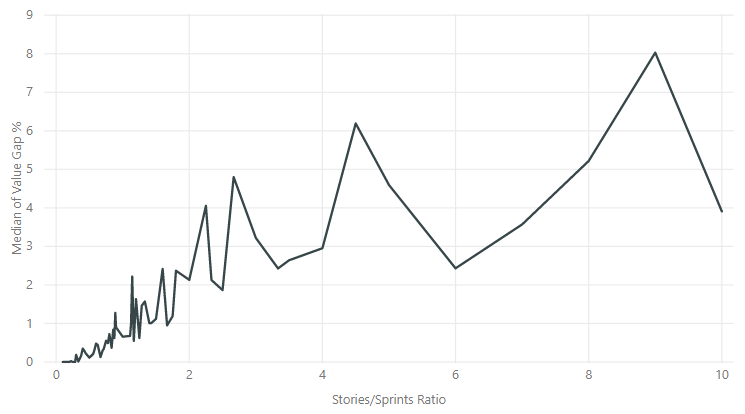
\includegraphics[width=\textwidth]{Figures/Results/annealing_value_gap_stories_sprints.png}
    \caption{Value Gap \% vs Stories/Sprints Ratio}
    \label{fig:value_gap_vs_stories_sprints}
\end{figure}

\begin{figure}[h!]
    \centering
    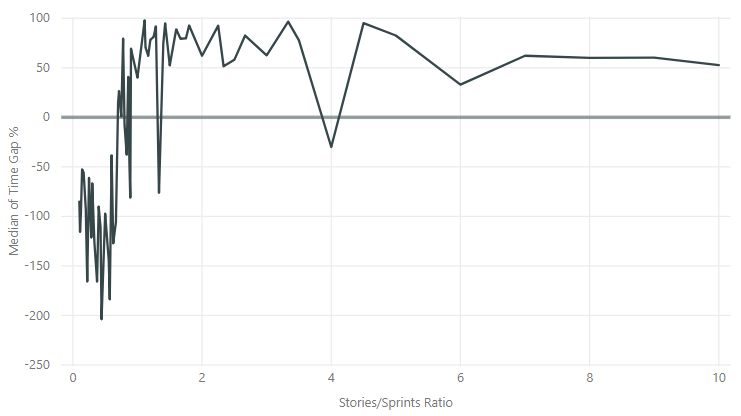
\includegraphics[width=\textwidth]{Figures/Results/annealing_time_gap_stories_sprints.png}
    \caption{Time Gap \% vs Stories/Sprints Ratio}
    \label{fig:time_gap_vs_stories_sprints}
\end{figure}